\documentclass[11pt]{article}
\usepackage[utf8]{inputenc}
\usepackage[T1]{fontenc}
\usepackage[a4paper,margin=1in]{geometry}
\usepackage{amsmath,amssymb}
\usepackage{graphicx}
\usepackage{microtype}
\usepackage{booktabs}
\usepackage[hidelinks]{hyperref}
\usepackage[round,authoryear]{natbib}
\usepackage{enumitem}
\usepackage{titlesec}
\titleformat{\section}{\large\bfseries}{\thesection}{0.6em}{}
\titleformat{\subsection}{\normalsize\bfseries}{\thesubsection}{0.6em}{}
\setlength{\parskip}{0.35em}
\setlength{\parindent}{0pt}

\title{\textbf{Frontier LLMs Add Almost No Information Beyond the Market Price,\\ and Two Years of Scaling Has Not Changed That}\\[0.4em]
\large A market-relative ``edge'' is Brier in disguise and the encompassing coefficient is too noisy to rank, which is why the gap went unmeasured; across 25 ForecastBench rounds (2024--2026) the bias-corrected information frontier models add beyond a liquid market price stays near zero and does not rise with scale, while human superforecasters on the one released human round clear the same bar by an order of magnitude}
\author{Vaticinus Research\thanks{The authors develop forecasting systems independently of this benchmark analysis and declare no other competing interests.}\\ \normalsize \texttt{vaticinus.com}}
\date{\today}

\begin{document}
\maketitle

\begin{abstract}
\noindent Probabilistic forecasters, including large language models (LLMs), are ranked almost entirely on the Brier score, which rewards a forecaster for reproducing an already-public market price. We ask what frontier LLMs actually add \emph{beyond} that free price, and find: almost nothing, and no more in 2026 than in 2024. On public, leak-free ForecastBench data spanning 25 resolved rounds (2024-07 to 2026-05; $1{,}256$ frontier-model configuration--rounds, $342$ configurations, $370{,}972$ resolved market forecasts), the bias-corrected incremental log-likelihood a model adds beyond a liquid market price is about $0.001$ nats, with a non-positive trend across two years and a dozen model generations from GPT-3.5 and Claude-2.1 to GPT-5.x and Claude-Opus-4.x (round-level slope $-0.004$ nats/yr, $95\%$ CI $[-0.008,-0.002]$; capability-axis slope $-0.0012$, $[-0.0020,-0.0006]$). That near-zero number is a statement about models only if the metric can be non-zero on this question class, so we anchor it with a positive control. On the one round with a released human track the same measure gives human superforecasters about $0.09$ nats, an order of magnitude above their own finite-sample floor, surviving the identical finite-sample correction and, decisively, a re-scoring of both groups on the \emph{same} (no-easier) questions ($+0.087$ nats, bootstrap CI excluding zero); the model null itself also survives an out-of-sample cross-fitted check. The control establishes that $\Delta$LL has dynamic range here, so the near-zero model value is a property of the models and not of a degenerate metric, and the $\sim\!75\times$ ratio we report as a single-round measurement, not a population estimate. We then explain why this gap went unmeasured: the two market-relative metrics the field has reached for cannot see it. The additive \emph{marginal edge} (a forecaster's proper score minus the price's) is Brier shifted by a per-question constant: rank-identical to Brier on all 25 rounds to machine precision ($\rho=1.000$, within-round constant SD $\le 6\times10^{-17}$), so on the real leaderboard it merely crowns the model that copied the price best. The forecast-encompassing coefficient $\beta_{\mathrm{fc}}$ is in turn too noisy to rank (split-half reliability $0.22$ against $0.87$ for Brier). The collinearity-robust object that does measure contribution is $\Delta$LL, which we use at the \emph{group} level, where it pools thousands of forecasts, not as a per-forecaster rank. The practical lesson for benchmark design is to report two separate axes, Brier for closeness to truth and bias-corrected $\Delta$LL for contribution beyond the priced consensus, and never to publish the marginal edge as a ranking. We concede the idea of market-relative scoring to prior work (Prophet Arena, the AIA Forecaster), which our negative result does not refute; the contribution here is the order-equivalence, the leak-free multi-round measurement, and the finding that scale has not populated the contribution axis. Externally submitted agentic research/tool systems sit modestly higher, a fragile signal we offer only as a hypothesis that contribution comes from research, not scale. The human comparison rests on the one released human round; we use it as a positive control on the metric rather than a population estimate, and mark it as such throughout.
\end{abstract}

\section{Introduction}

Language models now produce probabilistic forecasts at scale, and the community evaluates them with a small set of headline metrics: the Brier score \citep{brier1950}, sometimes the logarithmic score, and accuracy against a human crowd \citep{halawi2024,karger2024,lu2025}. These metrics share a blind spot. A proper score measures how close a forecast is to the truth, but on many questions the truth is already public in probability terms, because a liquid market or a large crowd has moved the implied probability close to where it will resolve. A forecaster who reads the price and reports it then scores almost as well as one who reasoned independently to the same number. Brier cannot tell the two apart, and the gap is visible for LLMs in the ForecastBench data \citep{karger2024}, where, as we show directly in Section~\ref{sec:dll}, the same model scores better on market questions when the crowd freeze value is supplied in the prompt than when it is not.

Two corrections present themselves, and a forecaster-evaluation literature already reaches for each. The first is to score the proper score \emph{relative} to the free prior, the \textbf{marginal edge}, which is the forecasting analogue of investment alpha and the basis of a market-aware evaluation frontier \citep{yang2025,alur2025}. The second is to estimate, with a forecast-encompassing regression, a coefficient $\beta_{\mathrm{fc}}$ on the forecaster's prediction after conditioning on the price, so that $\beta_{\mathrm{fc}}>0$ marks information the price does not contain \citep{fair1990,clements2010}. This paper asks whether either correction does what it is meant to, namely rerank a leaderboard by contribution rather than by closeness to a public number. On public ForecastBench data the answer for both is no, and the reasons are instructive.

Take the marginal edge first. The price enters the per-question edge $d_i^f = S(p^{\mathrm{ref}}_i,y_i) - S(p^f_i,y_i)$ only through $S(p^{\mathrm{ref}}_i,y_i)$, which depends on the question $i$ but not the forecaster $f$. It is a question main effect. Adding a per-question constant to every forecaster's edge changes the leaderboard's level, not its order. On a balanced panel the constant is global and $\mathrm{edge} = c - \mathrm{Brier}$, so the rankings coincide; on an unbalanced panel the naive edge ranking does differ from Brier, but only because forecasters answered different questions, and the difficulty adjustment that corrects that selection absorbs the price into a question fixed effect, leaving the adjusted edge ranking equal to the adjusted Brier ranking. This is a corollary of how skill scores relate to the underlying proper score \citep{murphy1973,wheatcroft2019} rather than a new theorem; our contribution here is to make it precise for the question-varying market price that the recent literature uses, and to verify it on data.

The encompassing coefficient is genuinely a different statistic, but it does not rescue the ranking either. The coefficient $\beta_{\mathrm{fc}}$ is not a relabeling of Brier, so in principle it could carry the price's information into the order. In practice it is too noisy to rank: re-estimated on random question halves, its rank reliability pooled across the 25 rounds is $0.22$ where Brier's is $0.87$, and on a single round its near-zero correlation with Brier ($\rho=0.06$, $p=0.50$) is what that noise produces rather than a clean second axis. Its much-discussed fall when a model copies the price turns out to be collinearity between the forecast and the price reallocating shared variance, not information disappearing.

The quantity that does measure contribution is robust to this collinearity: it is the incremental log-likelihood of the forecast beyond the price, $\Delta$LL, the improvement in fit from adding the forecaster's prediction to a model that already contains the price. It is the ensemble-improvement view of forecaster value \citep{satopaa2014,alur2025} expressed as a likelihood gain. On the ForecastBench LLM configurations $\Delta$LL is essentially zero, and supplying the price in the prompt does not lower it, because there is nearly nothing beyond the price for the model to lose. On the 23 human superforecasters $\Delta$LL is clearly positive, and the superforecaster median ensemble both adds information beyond the price and beats it on Brier. Closeness to truth and contribution beyond the priced consensus are two distinct axes, and on current models the second is close to empty.

So far the picture is one round, which invites the obvious objection that 2024-era models were simply not good enough. The 25-round ForecastBench panel answers it directly, because the benchmark re-runs a systematic battery of the day's frontier models every round, with release dates spanning GPT-3.5 and Claude-2.1 in 2023--24 through GPT-5.x, Claude-Opus-4.x, Gemini-3.x, Grok-4.x, DeepSeek, Qwen and Kimi generations in 2026. The measurement requires care, because an incremental likelihood is upward biased in finite samples and the late rounds have fewer resolved questions; once that bias is removed (Section~\ref{sec:trend}), the bias-corrected $\Delta$LL is about $0.001$ nats and its trend is non-positive (round-level slope $-0.004$ nats/yr, capability-axis slope $-0.0012$ nats/yr, both with confidence intervals below zero). The same correction, applied to the human superforecasters who answer far fewer questions and so face a larger bias, leaves them essentially unchanged at $\sim\!0.09$ nats; the human round thus acts as a positive control that the contribution axis is reachable, and the resulting $\sim\!75\times$ ratio is a single-round measurement, not an artifact of how the two groups are measured. The null is robust to leakage, which on market questions resolving after the freeze tends to favor the newer models. One group sits modestly higher, the externally submitted agentic research-and-tool systems, but the signal is fragile, so we offer ``contribution comes from research, not scale'' as a hypothesis, not a finding.

\paragraph{Contributions.}
\begin{enumerate}[leftmargin=1.4em,itemsep=2pt]
\item \textbf{The measurement.} On 25 leak-free ForecastBench rounds (2024--2026), the bias-corrected information frontier models add beyond a liquid market price is about $0.001$ nats and does not rise with scale: across two years and a dozen model generations (GPT-3.5 and Claude-2.1 to GPT-5.x and Claude-Opus-4.x) the trend is non-positive (round-level slope $-0.004$ nats/yr, $95\%$ CI $[-0.008,-0.002]$; capability-axis slope $-0.0012$, $[-0.0020,-0.0006]$), and the null survives an out-of-sample cross-fit. Human superforecasters on the one released human round clear the same bar by an order of magnitude under the identical finite-sample correction ($\sim\!0.09$ nats, a $\sim\!75\times$ gap that survives a same-questions control), so the near-zero model value is a property of the models, not a degenerate metric (Sections~\ref{sec:dll}, \ref{sec:trend}).
\item The collinearity-robust object that makes that measurement possible: the incremental log-likelihood $\Delta$LL of a forecast beyond the price, used at the group level, together with the finite-sample bias correction an incremental likelihood requires when resolved-question counts vary across rounds (Sections~\ref{sec:dll}, \ref{sec:trend}).
\item An explanation of why the gap went unmeasured: the two market-relative statistics the field reaches for cannot see it. The score-difference marginal edge is Brier shifted by a per-question constant, rank-identical to Brier on a balanced panel and to difficulty-adjusted Brier on an unbalanced one on all 25 rounds to machine precision, so on the real ForecastBench leaderboard it merely reproduces the Brier order and crowns the model that best copied the price (Sections~\ref{sec:obs}, \ref{sec:order}, \ref{sec:worked}); and the encompassing coefficient $\beta_{\mathrm{fc}}$ is too noisy to rank (split-half reliability $0.22$ against $0.87$ for Brier), its much-discussed copy-the-market signal being collinearity rather than lost information (Section~\ref{sec:beta}).
\item A two-axis reading for benchmark design: report Brier for closeness to truth and bias-corrected $\Delta$LL for contribution beyond the price; do not report the marginal edge as a ranking, and do not rank on a single-round $\beta_{\mathrm{fc}}$ (Section~\ref{sec:discussion}).
\end{enumerate}

\section{Related Work}

\paragraph{Skill scores and the underlying proper score.} The Brier Skill Score $1-\mathrm{BS}/\mathrm{BS_{ref}}$ is the standard improvement-over-baseline measure \citep{jolliffe2012}, and the verification literature has long studied how it relates to the proper score it is built from. \citet{murphy1973} decomposed the Brier score into reliability, resolution, and uncertainty; \citet{murphy1987} gave the general calibration and refinement framework. The reference in this tradition is a single statistical baseline such as climatology, and \citet{mason2004} and \citet{weigel2007} showed that the choice of reference and the structure of the skill score affect its expected value. \citet{wheatcroft2019} showed the ratio form is biased and small-sample-fragile and recommended reporting score differences, which we do, before showing that even the difference does not change a ranking. The decision-theoretic claim that what matters is improvement over the freely-available baseline is the distinction between a forecast's value and its skill \citep{murphy1993}.

\paragraph{When two proper scores agree on an ordering.} That a single proper score under-determines the comparison of forecasters, so that two forecasters can be equal on one score and differ on a finer comparison, is the subject of \citet{degroot1983}, \citet{dawid1986}, and \citet{schervish1989}; the underlying information ordering is Blackwell sufficiency \citep{blackwell1953}. A recent decision-theoretic ``informativeness gap'' \citep{feng2025} generalizes this comparison and recovers Blackwell informativeness when both predictors are calibrated, with an application to LLM forecasters. Our $\Delta$LL is one operational, likelihood-gain reading of ``forecaster refines the price'' relative to a fixed market reference, rather than the general decision-theoretic gap.

\paragraph{Proper scoring and calibration.} A skill measure must be built on a strictly proper rule to remain incentive-compatible \citep{gneiting2007jasa}, and the information a forecaster adds beyond a prior is the calibrated sharpness of \citet{gneiting2007jrssb}; the reliability/resolution decomposition that separates a forecast's calibration from the information it carries beyond a reference is made precise by \citet{brocker2009}, and our $\Delta$LL is the resolution-side, contribution component of that split.

\paragraph{Forecast combination and encompassing.} The encompassing regression we examine is a forecast-combination regression \citep{bates1969,granger1984,fair1990,clements2010}: $\beta_{\mathrm{fc}}$ is the weight on the forecaster relative to the price, and $\Delta$LL is the likelihood gain from that combination over the price alone. \citet{satopaa2014} give the information-diversity reason a less accurate forecaster can still hold information not in the crowd, which is what positive $\Delta$LL detects.

\paragraph{Edge over the crowd in human forecasting.} The Good Judgment Project defined forecaster value as improvement over the crowd \citep{mellers2014,mellers2015}, and \citet{atanasov2017} compared market prices against poll aggregates as alternative crowds, which motivates using the market price as the prior where one exists. That a \emph{selected} sub-crowd can beat the full crowd \citep{mannes2014} is why the superforecaster median ensemble, not the public aggregate, is the human comparator we use. Treating a raw price as a calibrated probability is itself an assumption \citep{wolfers2006}, to which we return in Section~\ref{sec:limits}.

\paragraph{LLM forecasting evaluation.} This literature reports mostly absolute Brier or accuracy against a crowd. \citet{zou2022} introduced an early neural forecasting benchmark; \citet{halawi2024} evaluate a retrieval-augmented system against the crowd aggregate; \citet{karger2024} introduce ForecastBench and rank on a difficulty-adjusted Brier; \citet{schoenegger2023} find GPT-4 below the crowd; \citet{lu2025} reports a frontier model beating the crowd on Brier but short of superforecasters. In each the crowd is a comparison target, not a per-question reference against which contribution is scored. Language models are also documented to be systematically overconfident \citep{kadavath2022,tian2023}, which is why a contribution measure such as $\Delta$LL, which rewards directional information rather than calibration, must be reported alongside a proper score rather than in place of it (Section~\ref{sec:discussion}). A complementary concern is that as models improve they increasingly correlate with the human consensus and so add less to a hybrid ensemble, the accuracy--correlation effect of \citet{jeddi2026}, which our finding that models track the market price restates in price terms.

\paragraph{Market-as-reference: the nearest prior art.} Prophet Arena \citep{yang2025} scores model advantage over an explicit market baseline and down-weights low-discrimination, already-priced questions through an IRT model; the AIA Forecaster \citep{alur2025} uses the market as the baseline and frames model value as information that diversifies a market ensemble. The idea of edge over the market is theirs, not ours. Our results are consistent with their designs and clarify why those designs take the form they do: both step outside the additive score difference that we show cannot rerank, the IRT weight by reweighting questions and the ensemble view by measuring incremental contribution. Our $\Delta$LL is the latter quantity made explicit at the group level, and it is a complement to Prophet Arena's question-level discrimination weight rather than a substitute, since a question can be highly discriminating yet fully priced and a low-discrimination question can still carry forecaster-specific signal. We stress that our order-equivalence does \emph{not} refute either system: both rank by reweighting questions (Prophet Arena's IRT) or by an ensemble-contribution view (the AIA Forecaster), not by the additive score difference we show is rank-equivalent to Brier. The target of that negative result is the naive market-edge column a benchmark designer might be tempted to publish, not these systems.

\section{The Marginal Edge and the Order-Equivalence}
\label{sec:metric}

\subsection{Setup}
Questions are indexed $i \in \{1,\dots,N\}$. Question $i$ has a binary outcome $y_i \in \{0,1\}$ (categorical and continuous cases extend through the ranked-probability score and the CRPS, whose reliability and resolution decomposition \citep{hersbach2000} is the proper analogue of the Murphy partition), a \textbf{reference prior} $p^{\mathrm{ref}}_i \in (0,1)$ that is a market price at a pre-fixed snapshot $t^{*}$, and a forecaster prediction $p_i \in (0,1)$. We use the Brier score $S(p,y)=(p-y)^2$ as the primary rule and the log score as a robustness check, both clipped at $\epsilon=10^{-3}$.

\subsection{The per-question edge}
The per-question marginal contribution of forecaster $f$ is
\[ d_i^f \;=\; S\!\left(p^{\mathrm{ref}}_i, y_i\right) - S\!\left(p^f_i, y_i\right), \]
positive when $f$ beats the price on question $i$. We use the difference of two proper scores rather than the skill-score ratio, which is biased and small-sample-fragile \citep{wheatcroft2019}; a difference of proper scores is also the object of the standard equal-predictive-accuracy test \citep{diebold1995}. The difference keeps proper incentives in $p^f$ because the reference term is exogenous to the forecaster, and that same exogeneity is what removes the price from any ranking.

\subsection{The order-equivalence}
\label{sec:obs}

\textbf{Proposition.} \emph{Write $A_i \equiv S(p^{\mathrm{ref}}_i,y_i)$, a quantity that depends on the question but not the forecaster.}
\begin{enumerate}[leftmargin=1.6em,itemsep=2pt,label=(\alph*)]
\item \emph{Balanced panel.} If every forecaster answers a common question set $\mathcal Q$, then each forecaster's mean edge is $\overline d^{\,f} = \frac1{|\mathcal Q|}\sum_{i\in\mathcal Q} A_i - \overline{\mathrm{Brier}}_f$, in which the first term is one constant shared by all forecasters. So $\overline d^{\,f}$ is a strictly decreasing affine function of $\overline{\mathrm{Brier}}_f$, and ranking by mean edge is identical to ranking by mean Brier, for any prior.
\item \emph{Unbalanced panel, difficulty-adjusted.} If forecasters answer different subsets and we estimate the difficulty-adjusted effect $\hat\alpha_f$ from the two-way forecaster$\,\times\,$question model $d_i^f = \mu + \alpha_f + \gamma_i + \varepsilon_i^f$ \citep{abowd1999}, then $A_i$ is collinear with the question dummies and is absorbed into $\hat\gamma_i$. The estimated $\hat\alpha_f$ is therefore the same as the one obtained with $-S(p^f_i,y_i)$ as the dependent variable, so the difficulty-adjusted edge ranking equals the difficulty-adjusted Brier ranking.
\end{enumerate}
Part (a) is one line of algebra. Part (b) is the Frisch--Waugh--Lovell absorption \citep{frisch1933,lovell1963} of any pure function of $i$ into the question effect. The naive unbalanced edge ranking does differ from Brier, but only through $\frac1{N_f}\sum_{i\in\mathcal Q_f} A_i$, which varies across forecasters solely because they chose different questions, which is selection and not skill relative to the price. The difficulty adjustment is the right remedy for that selection, and it removes the price along with it. The practical reading is that the marginal edge moves a leaderboard's level and not its order, so whatever the order encodes about the price, a score difference does not encode it. This is why the climatology-anchored skill-score tradition, which always uses a single constant reference, never had occasion to state it.

\section{The Order-Equivalence on Data}
\label{sec:order}
We use public and leak-free ForecastBench data \citep{karger2024}, distributed under CC BY-SA 4.0. The \textbf{LLM track} releases per-question forecasts for a systematic battery of the day's frontier models, re-run every round, across developers including Anthropic, Google, Meta, Mistral, OpenAI, xAI, DeepSeek, and others (zero-shot, scratchpad, news, and superforecaster prompts, with and without the freeze value supplied). We take the 29 processed rounds from 2024-07-21 to 2026-05-24 and keep the 25 in which enough market questions have resolved to estimate each configuration's statistics on at least $50$ rows; the remaining four are recent rounds awaiting resolution. This yields $1{,}256$ frontier-model configuration--rounds ($342$ distinct configurations) and $370{,}972$ resolved binary market forecasts. Within a round all configurations answer the same question set, so on the market sources each round is a balanced panel. The \textbf{human track} is released for the 2024-07-21 round only: 40 superforecasters and 500 public forecasters, of whom 23 superforecasters answer at least 20 market questions (56 distinct), a sparse and unbalanced panel. Forecasts are elicited at the freeze before resolution, so every round is leak-free by the benchmark's contamination-free design. A reference prior is a genuine probability only for market sources (manifold, metaculus, polymarket, infer); for data sources it is a raw series level, which we use only as a constant-prior implementation check. To orient the reader: the order-equivalence (this section) and the $\Delta$LL trend (Section~\ref{sec:trend}) are multi-round (25 rounds); the copy-the-market experiment, the human comparison, and the per-forecaster table (Sections~\ref{sec:dll}) use the single 2024-07-21 round, the only one with a released human track.

\paragraph{The identity holds every round, to machine precision.} On each of the 25 balanced LLM rounds the per-configuration constant $c_i^f = \overline{d}^{\,f} + \overline{\mathrm{Brier}}_f$ that Proposition (a) predicts to be forecaster-invariant is in fact identical across all configurations: its within-round standard deviation never exceeds $6.0\times10^{-17}$, fourteen orders of magnitude below the $10^{-3}$ at which Brier ranks resolve (Figure~\ref{fig:robust}a). The edge ranking therefore equals the Brier ranking exactly in every round ($\rho=1.000$, minimum $0.99999\!\dots$ across the 25). What was a single-round coincidence is a structural fact of the score difference, reconfirmed on two years of disjoint question sets. On the unbalanced human panel the naive edge ranking differs from Brier at $\rho = 0.358$, but the difficulty-adjusted forecaster effect computed from the edge $d$ and from negative Brier $-S(p^f,y)$ are the same to within $10^{-15}$ (maximum centered difference $1.1\times10^{-15}$ across the 23 forecasters), confirming Proposition (b): the reference is fully absorbed by the question fixed effect. The human leaderboard does reorder under the difficulty adjustment relative to raw Brier, but that reordering is the effect of adjusting for who answered which questions, and it owes nothing to the marginal-edge framing, since one obtains the identical result by difficulty-adjusting Brier with no reference at all.

\begin{figure}[t]
\centering
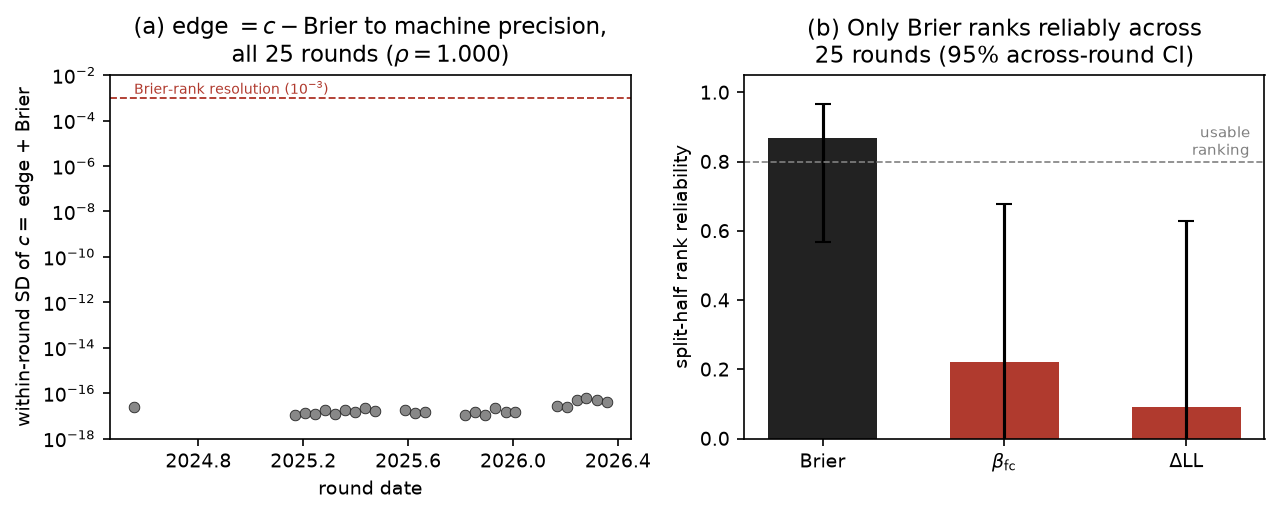
\includegraphics[width=0.92\linewidth]{out_mr/fig_robust.png}
\caption{The two negatives hold across 25 rounds. \textbf{(a)} The constant $c=$ edge $+$ Brier that Proposition (a) predicts to be forecaster-invariant has a within-round standard deviation of $\sim\!10^{-17}$ in every round, fourteen orders of magnitude below the $10^{-3}$ resolution of a Brier ranking, so the edge ranking equals the Brier ranking exactly ($\rho=1.000$) each round. \textbf{(b)} Split-half rank reliability pooled across the 25 rounds (bars are the across-round mean, whiskers the $95\%$ across-round interval): only Brier ($0.87$) clears the threshold for a usable individual ranking; the encompassing $\beta_{\mathrm{fc}}$ ($0.22$) and the incremental $\Delta$LL ($0.09$) do not rank individual configurations reliably.}
\label{fig:robust}
\end{figure}

\subsection{A worked example: who the marginal-edge leaderboard crowns}
\label{sec:worked}
The order-equivalence is easy to state abstractly and easy to underrate, so we make it concrete on the canonical board: the 130-configuration ForecastBench LLM leaderboard for 2024-07-21. Ranking these configurations by the marginal edge reproduces the Brier order to the digit (Table~\ref{tab:worked}; the edge and Brier ranks are byte-identical, $\rho=1.000$). What the edge ranking encodes about the market is nothing the Brier ranking did not already encode. Worse, on this round the liquid market price itself scores a Brier of $0.069$, better than all $130$ models, so every model's edge is \emph{negative}: the marginal-edge board ranks $130$ configurations that all lose to the market, ordered by how closely they tracked it. The configuration it crowns, GPT-4o with the freeze value supplied, was handed the market price in its prompt; $14$ of the top $15$ were likewise price-handed, and the top configuration's bias-corrected $\Delta$LL is $-0.0005$, that is, it adds nothing of its own. A market-relative leaderboard built on the marginal edge, advertised as ranking information beyond the market, here ranks price-copying and rewards the configuration that copied best.

The axis such a leaderboard means to measure lies elsewhere, and on current models it is nearly empty. Contribution beyond the price, $\Delta$LL, is decorrelated from Brier on this round ($\rho=0.01$), so the best price-tracker is not the largest contributor; and measured reliably by pooling each base model across all $25$ rounds, the contribution of even the most informative model (Meta-Llama-3.1-405B, $+0.013$ nats) is about seven times below the human superforecaster level ($0.091$), while the two lowest-Brier models on that pooled panel (Grok-beta and o3) sit at $+0.004$ and $-0.001$ nats, so the most accurate models are not the largest contributors. The lesson for a benchmark designer is concrete: do not publish a marginal-edge column believing it surfaces market-beating information. It is the Brier column under another name, and the contribution column it is mistaken for is both decorrelated from it and, on today's models, near-empty.

\begin{table}[t]\centering
\small
\begin{tabular}{rlrrr}
\toprule
rk & configuration (top 10 by marginal edge) & Brier & edge & $\Delta\mathrm{LL}_{\mathrm{adj}}$\\
\midrule
1 & GPT-4o (scratchpad, freeze) & 0.100 & $-0.030$ & $-0.0005$\\
2 & GPT-4-Turbo (scratchpad, freeze) & 0.113 & $-0.043$ & $-0.0002$\\
3 & Claude-3.5-Sonnet (scratchpad, freeze) & 0.115 & $-0.046$ & $+0.0030$\\
4 & GPT-4-Turbo (zero-shot, freeze) & 0.117 & $-0.047$ & $+0.0001$\\
5 & GPT-4o (scratchpad, news, freeze) & 0.119 & $-0.050$ & $+0.0046$\\
6 & GPT-4-0613 (zero-shot, freeze) & 0.122 & $-0.052$ & $+0.0039$\\
7 & GPT-4-Turbo (scratchpad, news, freeze) & 0.124 & $-0.054$ & $-0.0007$\\
8 & Gemini-1.5-Flash (zero-shot, freeze) & 0.132 & $-0.063$ & $+0.0006$\\
9 & Claude-3.5-Sonnet (zero-shot, freeze) & 0.133 & $-0.063$ & $+0.0065$\\
10 & Claude-3-Opus (zero-shot, freeze) & 0.133 & $-0.064$ & $+0.0042$\\
\bottomrule
\end{tabular}
\caption{The real ForecastBench 2024-07-21 LLM leaderboard, top 10 of 130 by marginal edge. The edge rank equals the Brier rank byte-for-byte across all 130 ($\rho=1.000$). The market price scores Brier $0.069$, better than every model, so all edges are negative. ``freeze'' marks configurations handed the market price in the prompt: $14$ of the top $15$ are price-handed, and the board's winner adds $\Delta\mathrm{LL}_{\mathrm{adj}}=-0.0005$ beyond the price. Per-configuration $\Delta\mathrm{LL}$ is individually noisy (Section~\ref{sec:beta}) and is shown only to make the point that the top of the edge board sits at $\approx\!0$ contribution; across the panel $\rho(\Delta\mathrm{LL},-\mathrm{Brier})=0.01$.}
\label{tab:worked}
\end{table}

\section{The Encompassing Coefficient Also Fails to Rank}
\label{sec:beta}
The coefficient $\beta_{\mathrm{fc}}$ from the forecast-encompassing logit $y_i = \Lambda(\beta_0 + \beta_{\mathrm{ref}} z^{\mathrm{ref}}_i + \beta_{\mathrm{fc}} z^f_i)$, with $z=\mathrm{logit}(p)$, is not an affine transform of Brier, so unlike the marginal edge it is not ruled out a priori as a ranking. We estimated it per configuration on the 256 market questions, with standard errors clustered by question, and find three reasons it cannot serve as a leaderboard.

First, it is too noisy to rank. Splitting the questions into halves and re-estimating, the rank correlation of $\beta_{\mathrm{fc}}$ across halves averages $0.23$ on this round, against $0.96$ for Brier (Figure~\ref{fig:neg}b); only $18\%$ of configurations have a $\beta_{\mathrm{fc}}$ distinguishable from zero. This is not a property of the one round: pooled across all 25 rounds the split-half rank reliability of $\beta_{\mathrm{fc}}$ is $0.22$ (across-round SD $0.28$), against $0.87$ for Brier, while the incremental $\Delta$LL is likewise unreliable as a per-configuration rank ($0.09$) even though, as Section~\ref{sec:dll} shows, it is the right instrument at the group level (Figure~\ref{fig:robust}b). Second, its small correlation with Brier across configurations ($\rho = 0.06$, $p = 0.50$, $95\%$ bootstrap interval $[-0.11, 0.23]$) cannot be read as orthogonality. The reliability of $\beta_{\mathrm{fc}}$, the share of its between-configuration variance that is signal rather than sampling noise, is $0.18$; by the classical attenuation relation \citep{spearman1904} a statistic that is mostly noise is mechanically near-uncorrelated with everything, so $\rho = 0.06$ is what one would observe whether $\beta_{\mathrm{fc}}$ were truly orthogonal to Brier or not. The data simply cannot resolve a second axis at this sample size. Third, the apparent copy-the-market effect on $\beta_{\mathrm{fc}}$ is a collinearity artifact, which we show next.

\section{What Measures Contribution Beyond the Price}
\label{sec:dll}
The collinearity-robust measure of information a forecaster adds beyond the price is the incremental log-likelihood
\[ \Delta\mathrm{LL} \;=\; \tfrac1N\big[\,\mathrm{LL}(y \mid z^{\mathrm{ref}}, z^{f}) - \mathrm{LL}(y \mid z^{\mathrm{ref}})\,\big], \]
the per-forecast gain in fit from adding the forecaster's prediction to a model that already contains the price. Because it measures fit improvement rather than the partition of shared variance between two regressors, it is insensitive to the collinearity that destabilizes $\beta_{\mathrm{fc}}$ when a forecast tracks the price. It is the ignorance-score gain of \citet{roulston2002} relative to the price. We use $\Delta\mathrm{LL}$ only as a \emph{group-level} contribution estimate (for the battery, the human cohort, and the calendar trend, each pooling thousands of forecasts), not as a per-configuration ranking: at the single-forecaster level it is as unreliable as $\beta_{\mathrm{fc}}$ (pooled split-half $0.09$; Section~\ref{sec:beta}), so we never rank individual forecasters by it.

\paragraph{The copy-the-market experiment, read correctly.} ForecastBench ran 46 configurations as matched pairs that differ only in whether the market freeze value was supplied in the prompt, across 17 distinct base models. Supplying the price has a clear and consistent effect on what a model does and on its Brier: the distance to the price $|p-p^{\mathrm{ref}}|$ falls (family-median $-0.077$, every one of the 17 families, sign-test $p<0.001$) and Brier improves (family-median $-0.033$, every family). The raw $\beta_{\mathrm{fc}}$ falls as well (family-median $-0.19$), which one is tempted to read as the model adding less of its own information. That reading is wrong. The variance-inflation factor between the forecast and the price rises from $1.3$ to $1.6$ when the price is supplied, and the $\beta_{\mathrm{ref}}\!\uparrow$, $\beta_{\mathrm{fc}}\!\downarrow$ pattern is the signature of collinearity reallocating shared explanatory power from the now-redundant forecaster regressor to the price. The collinearity-robust $\Delta$LL does not fall: it is flat to slightly higher (family-median $+0.002$; lower in only $1$ of $17$ families). Both before and after the prompt manipulation, $\Delta$LL is essentially zero ($0.0008$ then $0.0028$ nats), so there is almost no information beyond the price for the model to lose. Supplying the price does not degrade a contribution; it reveals that there was little contribution to begin with (Figure~\ref{fig:pos}b). This also resolves an ambiguity in $|p-p^{\mathrm{ref}}|$ as a measure of copying, which on its own cannot separate copying from correct updating on a good prior: here $\Delta$LL is near zero, so the convergence to the price is not the model contributing independent information.

\paragraph{LLMs against superforecasters.} Measured by $\Delta$LL, the 130 LLM configurations add almost nothing beyond a liquid market price (mean $0.0018$ nats per forecast, Figure~\ref{fig:pos}a), and $\Delta$LL is essentially uncorrelated with Brier ($\rho=0.01$), so a better Brier among these models does not indicate more information beyond the price; it indicates closer tracking of it. The human superforecasters are different. Pooled across the 23 forecasters, $\Delta$LL is $0.08$ nats per forecast, and the superforecaster median ensemble adds $0.13$ nats on the 56 market questions while beating the market on Brier ($0.087$ against $0.131$). The two findings together say that on this round closeness to truth and contribution beyond the price come apart, and that current LLMs sit at the price while superforecasters move away from it with information. We report the human result as a single-round, selected-sample finding (Section~\ref{sec:limits}), not a population estimate. The reported $\Delta$LL values here are the raw in-sample figures; because the humans answer far fewer questions than the LLM configurations, a like-for-like comparison must remove the finite-sample bias of an incremental likelihood, which we do in Section~\ref{sec:trend}; the gap not only survives but widens, because the correction is large for the few-question humans yet they remain near $0.09$ nats while the models fall to $\sim\!0.001$.

\begin{figure}[t]
\centering
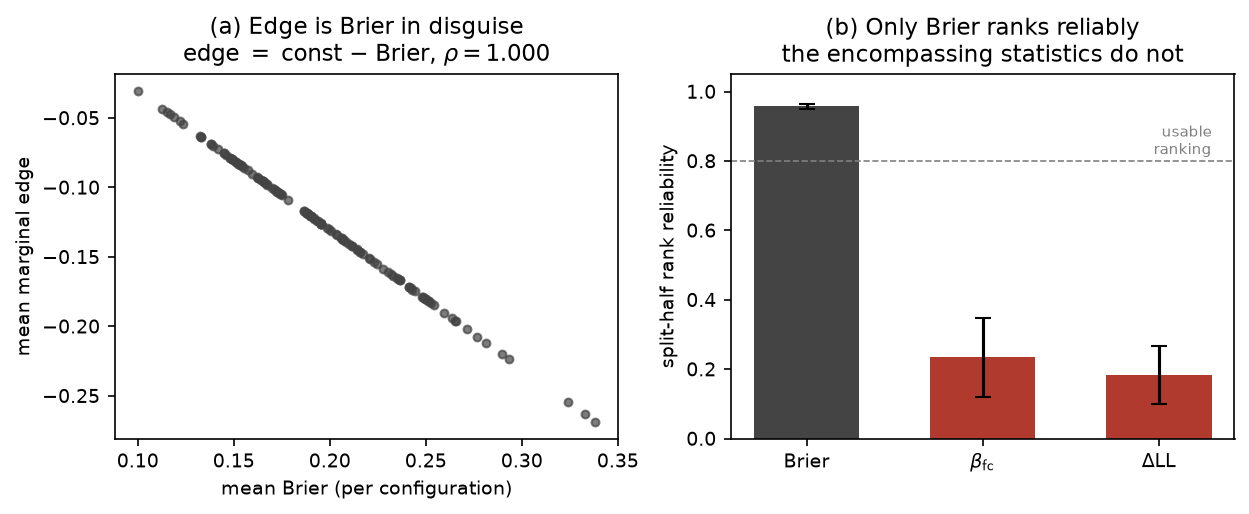
\includegraphics[width=0.92\linewidth]{out_llm/fig_negatives.png}
\caption{Neither correction reranks. \textbf{(a)} On the balanced 130-configuration LLM panel the marginal edge equals a constant minus Brier, so the edge ranking is the Brier ranking ($\rho=1.000$). \textbf{(b)} Re-estimating each statistic on random halves of the questions, only Brier produces a stable ranking (split-half rank reliability $0.96$); the encompassing $\beta_{\mathrm{fc}}$ ($0.23$) and the incremental log-likelihood $\Delta$LL ($0.18$) do not rank individual configurations reliably on one round.}
\label{fig:neg}
\end{figure}

\begin{figure}[t]
\centering
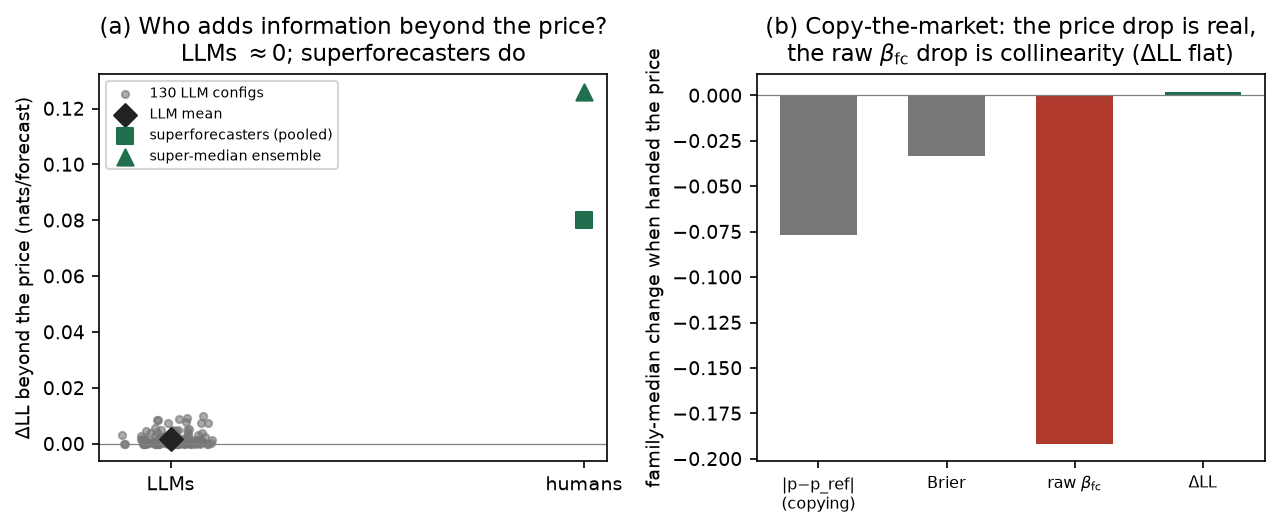
\includegraphics[width=0.96\linewidth]{out_llm/fig_positive.png}
\caption{Information beyond the price. \textbf{(a)} The incremental log-likelihood $\Delta$LL beyond the market price: the 130 LLM configurations cluster near zero, while pooled superforecasters ($0.08$ nats) and their median ensemble ($0.13$ nats) add real information. \textbf{(b)} In the copy-the-market experiment, supplying the price genuinely makes models copy it and lowers their Brier (left two bars, family-median changes), and it lowers the raw $\beta_{\mathrm{fc}}$, but the collinearity-robust $\Delta$LL is flat, so the $\beta_{\mathrm{fc}}$ drop is variance reallocation rather than lost information.}
\label{fig:pos}
\end{figure}

\paragraph{The human encompassing result.} For completeness, the pooled encompassing regression on the 23 superforecasters gives a positive forecaster coefficient ($\beta_{\mathrm{fc}}=0.62$, question-clustered $p=0.005$, wild cluster bootstrap-$t$ $p=0.0001$, pairs cluster bootstrap interval $[0.29,1.41]$) with the price coefficient not distinguishable from zero, consistent with the positive $\Delta$LL above. Because the per-forecaster $\beta_{\mathrm{fc}}$ is unreliable on one round (Section~\ref{sec:beta}), we treat this pooled coefficient as corroborating the $\Delta$LL finding for superforecasters as a group, not as a per-forecaster ranking. Table~\ref{tab:results} lists the per-forecaster numbers, with the difficulty-adjusted $\hat\alpha_f$ shown for reference; by Section~\ref{sec:order} that column is difficulty-adjusted Brier and carries no price information.

\begin{table}[t]\centering
\small
\input{out/results_table_v3.tex}
\caption{Market-track superforecasters, ordered by Brier rank. ``edge'' is the raw mean edge; $\hat\alpha_f$ is the difficulty-adjusted forecaster effect, which by Section~\ref{sec:order} equals difficulty-adjusted negative Brier and carries no price information; $^\ast$ marks the 7 forecasters with a positive edge surviving Benjamini--Hochberg control \citep{benjamini1995} at $q=0.10$. Labels F01--F23 anonymized; 56 market questions, single round.}
\label{tab:results}
\end{table}

\section{Two Years of Frontier Models Do Not Fill the Contribution Axis}
\label{sec:trend}
The single-round result, that LLMs sit at the price while humans do not, leaves open whether the contribution axis is empty in principle or merely empty for 2024-era models. ForecastBench answers this directly, because it re-runs a battery of the day's frontier models every round. Across the 25 rounds the systematic battery spans GPT-3.5-Turbo and Claude-2.1 (late 2023) through GPT-5.x, Claude-Opus-4.x, Gemini-3.x, Grok-4.x, and the DeepSeek, Qwen, and Kimi generations of 2026: two years of capability growth measured against the same kind of liquid market price each round.

\paragraph{A finite-sample bias must be removed first.} The in-sample $\Delta$LL is upward biased, and the bias is not uniform across rounds. Adding the forecast regressor to the price-only logit always raises the in-sample likelihood, and under the null that the forecast carries nothing beyond the price the likelihood-ratio statistic $2N\,\Delta\mathrm{LL}$ is asymptotically $\chi^2_1$ with mean $1$, so $\mathbb{E}[\Delta\mathrm{LL}]=\tfrac{1}{2N}$ even when there is no information to find. This bias is largest where $N$ is smallest, and $N$ falls sharply over the panel: the number of resolved market questions per round drops from $\sim\!250$ in 2024--25 to $\sim\!40$--$100$ in 2026 (correlation of questions-per-round with date $-0.84$), exactly where the newest models sit. The raw $\Delta\mathrm{LL}$ therefore flatters recent rounds. We remove the null bias, $\Delta\mathrm{LL}_{\mathrm{adj}} = \Delta\mathrm{LL} - \tfrac{1}{2N}$, and, crucially, apply the identical correction to the human numbers, whose forecasters answer only $\sim\!28$ questions each and so carry a \emph{larger} per-unit bias than the LLM configurations, which answer $\sim\!250$.

\paragraph{Corrected, the contribution is near zero and does not rise.} The bias correction removes most of the apparent model contribution: the battery's mean $\Delta\mathrm{LL}_{\mathrm{adj}}$ is $0.0012$ nats, down from a raw $0.0046$, i.e.\ roughly three-quarters of the naive figure was finite-sample artifact. The trend is, if anything, downward: the round-level slope is $-0.0040$ nats/yr (bootstrap $95\%$ CI $[-0.0078,-0.0017]$), the question-weighted slope is $-0.0020$ ($[-0.0078,+0.0002]$), and dropping the five thinnest rounds gives $-0.0035$ ($[-0.0079,-0.0008]$); no specification produces a positive trend (the raw $+0.0009$, $p=0.57$, was itself the small-$N$ bias). The capability axis tells the same story: ordering the $324$ configurations by model release date, the bias-corrected slope is $-0.0012$ nats/yr (base-model-clustered $95\%$ CI $[-0.0020,-0.0006]$), with models released on or before mid-2024 at $+0.0014$ nats and those released in 2026 at $-0.0024$ (Figure~\ref{fig:trend}). As an equivalence reading \citep{lakens2017}, the primary round-level slope's upper confidence bound is itself negative ($-0.0017$ nats/yr), so the data support no positive trajectory toward the human level at all; even the single most favorable specification (the question-weighted fit) has an upper bound near zero, under which closing the $\sim\!0.09$-nat gap would still take more than a century. The data exclude any approach to the human contribution on a relevant horizon. The level and slope are insensitive to the probability-clipping bound: at $\epsilon\in\{10^{-2},10^{-3},10^{-4}\}$ the bias-corrected level is $0.0011$ nats and the slope is $-0.004$ nats/yr throughout.

\paragraph{The null does not depend on the analytic correction.} Because the $1/2N$ adjustment is a first-order asymptotic and the late rounds are small, we re-estimate the battery contribution with a cross-fitted, out-of-sample $\Delta\mathrm{LL}$: fit the price-only and price-plus-forecast logits on one half of the questions, score the log-likelihood gain on the held-out half, and average symmetrically. This carries no in-sample optimism and needs no analytic correction. On the anchor round it gives $-0.001$ nats, matching the $1/2N$-corrected in-sample $+0.001$, so the near-zero model contribution is a property of the forecasts and not an artifact of the bias adjustment. The same cross-fit cannot validate the \emph{human} number, whose forecasters answer far too few questions to hold out a two-regressor logit (Section~\ref{sec:limits}); the human side is instead anchored by its order-of-magnitude margin over its own bias and by the matched-question control above.

\paragraph{The human contribution survives the same correction; the gap is not an estimator artifact.} Applying $\Delta\mathrm{LL}_{\mathrm{adj}}$ to the superforecasters, who answer far fewer questions and so face the larger bias, barely moves them: the per-forecaster mean falls only from $0.109$ to $0.091$ nats (bootstrap $95\%$ CI $[0.060,0.124]$), and the median ensemble from $0.126$ to $0.117$. The same operation that collapses the model number by three-quarters leaves the human number essentially intact, because the human gain is real signal an order of magnitude above its sampling bias whereas the model gain was mostly the bias. After the identical, apples-to-apples correction the human-to-LLM ratio is about $75\!:\!1$ ($0.091$ against $0.0012$), wider than the raw comparison and now demonstrably not a consequence of the two groups answering different numbers of questions. We read this human round as a positive control, not as a population estimate of human-over-model skill: its role is to show that $\Delta\mathrm{LL}$ is reachable on this question class, which one clean, bias-corrected, difficulty-matched instance establishes, and the $75\!:\!1$ figure is that instance rather than a law the model null depends on.

\paragraph{The gap is not a question-selection artifact either.} Beyond the question \emph{count}, the two groups answer different question \emph{sets} (the superforecasters $56$ market questions, the battery $256$), and a natural objection is that the human-answered subset is simply easier to beat the price on. It is not. Scored on the same $56$ questions, the human-answered set is if anything marginally harder than the full panel (mean $|p^{\mathrm{ref}}-0.5|$ of $0.357$ versus $0.393$), and on that common set the bias-corrected superforecaster contribution is $+0.084$ nats while the $130$-configuration battery's is $-0.003$ nats: negative, i.e.\ the models slightly \emph{worsen} on the price exactly where the humans contribute most. The matched gap is $+0.087$ nats (question-bootstrap $95\%$ CI $[+0.004,+0.177]$, excluding zero). The contribution gap is therefore a property of the forecasters, not of which questions each group was scored on; what a single human round leaves open is round-to-round variation in the human level (Section~\ref{sec:limits}), not within-round question selection.

\paragraph{The null is robust to leakage.} A non-positive trend is hard to attribute to contamination. Each forecast is frozen before its question resolves, so within a round the panel is leak-free by construction; across rounds, a later model carries a larger training cutoff, which on a market question resolving after the freeze tends to raise a model's raw accuracy. Its effect on $\Delta\mathrm{LL}$, accuracy \emph{beyond the price}, is weaker and of ambiguous sign, since knowledge that pulls the model toward the outcome also tends to pull it toward the price; but to whatever extent leakage moves $\Delta\mathrm{LL}$ at all it favors the newer models, so a flat-to-declining trend is not naturally produced by contamination. The reading that current models add almost nothing beyond a liquid price is, if anything, charitable to the newer ones.

\paragraph{A hypothesis on what would move it: research, not scale.} One group sits modestly higher: the externally submitted agentic systems (research-and-tool pipelines and ensembles entered by outside teams), present in 13 rounds. At the configuration level their bias-corrected $\Delta\mathrm{LL}_{\mathrm{adj}}$ averages $0.0040$ nats against the battery's $0.0012$ (Welch $p=0.04$). We do not lean on this. The per-round signal is fragile: its mean falls to essentially zero when the single best round is removed, its calendar trend is not significant ($p=0.17$), and these systems are the most leakage-exposed in the data, since several query the live web. We therefore offer ``contribution comes from research the price has not absorbed, not from model scale'' as a hypothesis consistent with the human result, not as a finding. What the data do establish is the negative: raw model scale, over two years and a dozen generations, has not climbed onto the contribution axis.

\begin{figure}[t]
\centering
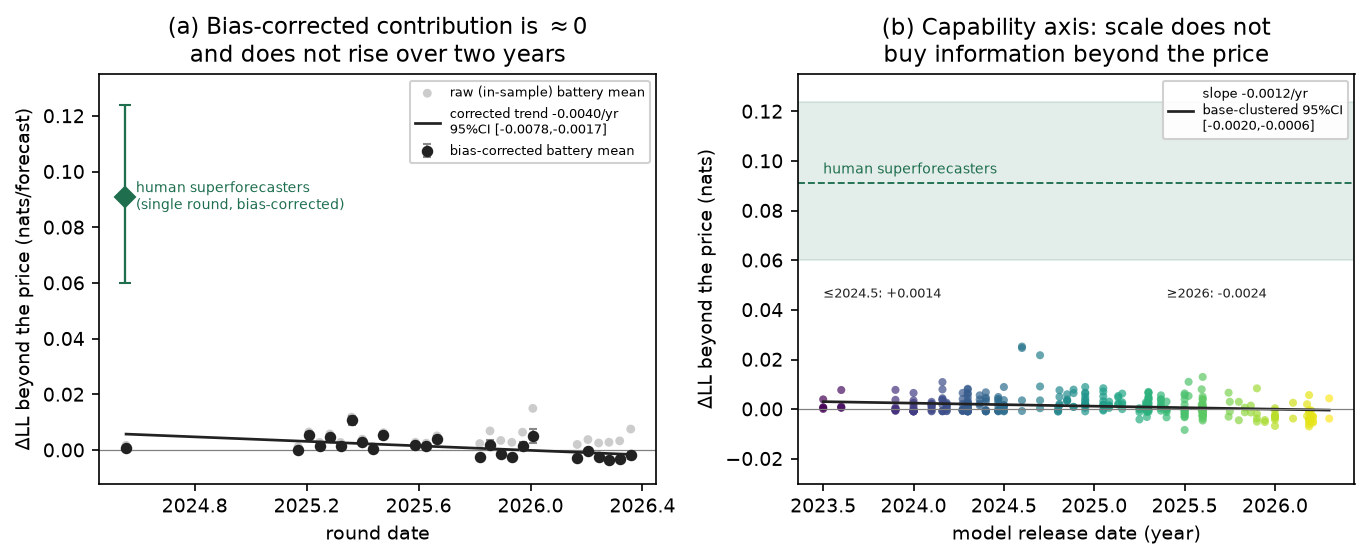
\includegraphics[width=0.96\linewidth]{out_mr/fig_trend.png}
\caption{The open question, answered. \textbf{(a)} Per-round $\Delta$LL beyond the price for the frontier-model battery: the raw in-sample mean (faded) is inflated by a finite-sample bias that is largest in the small late rounds; the bias-corrected mean (black, with across-configuration standard errors) is near zero with a non-positive trend ($-0.0040$ nats/yr, $95\%$ CI $[-0.0078,-0.0017]$). The single-round human superforecaster level (green diamond, with bootstrap CI), measured with the identical bias correction, sits $\sim\!75\times$ higher. \textbf{(b)} The capability axis: each of $324$ configurations by model release date; the bias-corrected slope is negative ($-0.0012$ nats/yr, base-model-clustered $95\%$ CI $[-0.0020,-0.0006]$), with the human band an order of magnitude above. Scale does not buy information beyond the price.}
\label{fig:trend}
\end{figure}

\section{Discussion}
\label{sec:discussion}
A forecasting leaderboard can measure two different things. One is closeness to the truth, which Brier measures and which the marginal edge measures again, since it is Brier shifted by a per-question constant. The other is contribution beyond the priced consensus, which $\Delta$LL measures and which the encompassing coefficient tries and fails to measure reliably on a single round. The recent push toward edge-over-market evaluation has been an attempt to get the second axis out of an operation that lives on the first, and our results say plainly why that cannot work in the score-difference form and is hard in the coefficient form. For a downstream user who wants the best probabilities to act on, closeness to truth is the right axis, and Brier remains the metric. For a user who wants to know whether a forecaster would improve an ensemble that already contains the market, contribution beyond the price is the right axis, and $\Delta$LL is the metric; this is the question the AIA ensemble framing also asks \citep{alur2025}. The two should be reported as separate columns, and the marginal edge should not be reported as a ranking at all: on the real ForecastBench leaderboard it reproduces the Brier order and crowns the model that best copied the market price (Section~\ref{sec:worked}).

\paragraph{Why $\Delta$LL and not the coefficient.} $\Delta$LL is a likelihood-ratio statistic that is robust to the forecast tracking the price, which is exactly the regime in which a market-relative metric is needed. It still requires a fixed question set, because on an open venue where forecasters choose questions a contribution measure rewards answering only where the price is expected to be wrong, which is prior-error harvesting rather than knowledge. It also requires pairing with a calibration check, because a contribution measure rewards directionally useful information and does not by itself penalize overconfidence; a model that is informative about direction but badly calibrated can show positive $\Delta$LL while being a poor standalone forecaster. And it requires the reference to be operator-fixed per question, since where several candidate priors exist the choice of reference is itself a degree of freedom a forecaster could exploit.

\paragraph{The state of current models.} The contribution axis is nearly empty for LLMs, and Section~\ref{sec:trend} shows this is not an artifact of model vintage or of the metric: across two years and the frontier releases of 2024--2026 the bias-corrected contribution stays near zero with a non-positive trend, about $75\times$ below the human level under the identical correction. LLMs sit at the market price, and supplying them the price simply moves them onto it more tightly, improving their Brier without adding information. The superforecasters are the positive control that the axis is not empty in principle, a role a single clean human round is enough to fill, and the agentic research systems point the same way: doing research the price has not absorbed moves a forecaster off the price with real information, and scaling the model that reads the price does not. Whether thinner and less efficient markets, or tool-using model systems rather than the models alone, populate the axis more fully is the natural next question; the evidence here is that raw capability growth, the lever the field has actually pulled, has not.

\section{Limitations}
\label{sec:limits}
\begin{enumerate}[leftmargin=1.4em,itemsep=2pt]
\item \textbf{What is multi-round, and what is not.} The order-equivalence (Sections~\ref{sec:obs}, \ref{sec:order}) is an algebraic identity and is confirmed on all 25 rounds; the unreliability of $\beta_{\mathrm{fc}}$, the near-zero LLM $\Delta$LL, and the flat capability trend (Section~\ref{sec:trend}) are now multi-round. The \emph{human} results (the positive superforecaster $\Delta$LL, the encompassing coefficient, and the per-forecaster table) remain single-round, because ForecastBench released a human track only for 2024-07-21. We use the human round as a positive control on the metric, not as a population estimate: its job is to establish that $\Delta$LL is reachable on this question class, which one clean, bias-corrected, difficulty-matched instance does, and on which the model contribution null does not depend. Further released human tracks would upgrade the $\sim\!75\times$ ratio from a single-round measurement to a population estimate, and that is the first thing we would add; but the paper's thesis, the near-zero model contribution and its flat trend across scale, stands without it.
\item \textbf{The capability axis has non-independent units; the bias correction is first-order.} The per-model release-date regression in Section~\ref{sec:trend} pools configurations that recur across rounds, so we report a base-model-clustered bootstrap interval rather than a naive $p$-value, and corroborate it with the round-level trend, whose 25 units are far less dependent (residual lag-1 autocorrelation is small). The finite-sample correction $\Delta\mathrm{LL}-\tfrac1{2N}$ is the first-order null-mean adjustment; it is the same quantity an AIC penalty targets, and an out-of-sample split would serve the same purpose, but on the smallest rounds a residual higher-order bias may remain. The agentic-systems comparison is heterogeneous, thin per round, partly tool-using, and not robust to dropping its best round, so we report it as a hypothesis, not an estimate.
\item \textbf{One liquid-prior regime.} The near-zero LLM contribution is measured against liquid market prices (manifold, metaculus, polymarket, infer). Thinner or less efficient markets, or non-market questions where no priced consensus exists, could leave more room for a model to contribute, and the result should not be read as a statement about language-model forecasting in the absence of a good price.
\item \textbf{The price is taken as a probability.} We treat the raw market price as a calibrated probability. Prices are known to be biased probability estimates \citep{wolfers2006}, with documented regularities such as the favorite--longshot bias \citep{snowberg2010}, so part of the superforecaster $\Delta$LL may be the freely-recoverable correction of a known price bias rather than private information. This is a ceiling on how much of the human contribution is genuinely private. We attempted to net this out by recomputing $\Delta$LL beyond an out-of-fold recalibrated price, but at one round's question count the recalibration injects enough reference noise to inflate $\Delta$LL spuriously for \emph{both} groups (it lifts the no-edge LLM battery to an artifactual $0.05$ nats), so the private-versus-recoverable decomposition is inconclusive here; the price's own recoverable miscalibration is in any case modest (out-of-fold recalibration improves its Brier only from $0.056$ to $0.047$), bounding how much of the human edge could be mere de-biasing. The mapping from a price to a probability is itself only a partial-identification bound \citep{manski2006}.
\item \textbf{Reflexive questions.} Several market sources resolve on a market or crowd state, in which case contribution beyond the price is partly a bet on the price's own future error rather than on an exogenous outcome. We did not separate exogenous from reflexive questions, and a clean version of the contribution measure would exclude or flag the reflexive case.
\item \textbf{Human sample is sparse and selected.} The human track is 23 superforecasters on 56 questions, with resolved questions easier than unresolved ones (mean $|p^{\mathrm{ref}}-0.5|$ $0.33$ against $0.25$, Mann--Whitney $p=0.018$). The cross-group difficulty confound this raises is addressed directly in Section~\ref{sec:trend} by scoring both groups on the common 56 questions (the gap survives at $+0.087$ nats, bootstrap CI excluding zero); what remains is the single-round nature of the human track, not within-round selection. The superforecaster $\Delta$LL is robust to question-clustered and bootstrap inference but remains a selected single-round result.
\end{enumerate}

\paragraph{Reproducibility.} {\sloppy All numbers are produced from public ForecastBench data (CC BY-SA 4.0). The single-round LLM analyses (reliability, split-half, collinearity-robust $\Delta$LL, copy-the-market pairs) are in \texttt{llm\_edge.py} and \texttt{llm\_edge2.py}; the human track in \texttt{revise\_edge\_v3.py}; the 25-round extension (the per-round order-equivalence to machine precision, the pooled reliabilities, the calendar and capability-axis $\Delta$LL trends, and the agentic-systems comparison) in \texttt{multiround.py}, the finite-sample bias correction, the slope confidence intervals, the base-model-clustered capability slope, and the apples-to-apples human comparison in \texttt{multiround\_rev.py}, the matched-question human-vs-model control in \texttt{matched\_question.py}, the clipping-sensitivity check in \texttt{eps\_sens.py}, the worked-example leaderboard in \texttt{worked\_example.py}, with figures in \texttt{mr\_figs.py}; outputs in \texttt{out\_llm/}, \texttt{out/}, and \texttt{out\_mr/}. The order-equivalence checks, including $\rho=1.000$ every round with within-round constant SD $\le 6\times10^{-17}$ and the $1.1\times10^{-15}$ Frisch--Waugh--Lovell equivalence on the human panel, are computed and committed in those scripts. The scripts and the derived per-round and per-configuration tables are released with the paper; the underlying forecasts are the public ForecastBench processed sets.\par}

\begin{thebibliography}{99}
\setlength{\itemsep}{1pt}
\bibitem[Abowd et al.(1999)]{abowd1999} Abowd, J. M., Kramarz, F., \& Margolis, D. N. (1999). High Wage Workers and High Wage Firms. \emph{Econometrica}, 67(2), 251--333.
\bibitem[Alur et al.(2025)]{alur2025} Alur, R., Stadie, B. C., Kang, D., Chen, R., McManus, M., Rickert, M., Lee, T., Federici, M., Zhu, R., Fogerty, D., Williamson, H., Lozinski, N., Linsky, A., \& Sekhon, J. S. (2025). \emph{AIA Forecaster: Technical Report.} arXiv:2511.07678.
\bibitem[Atanasov et al.(2017)]{atanasov2017} Atanasov, P., Mellers, B., Tetlock, P., et al. (2017). Distilling the Wisdom of Crowds: Prediction Markets vs.\ Prediction Polls. \emph{Management Science.}
\bibitem[Bates \& Granger(1969)]{bates1969} Bates, J. M., \& Granger, C. W. J. (1969). The Combination of Forecasts. \emph{Operational Research Quarterly}, 20(4), 451--468.
\bibitem[Benjamini \& Hochberg(1995)]{benjamini1995} Benjamini, Y., \& Hochberg, Y. (1995). Controlling the False Discovery Rate. \emph{JRSS B}, 57(1), 289--300.
\bibitem[Blackwell(1953)]{blackwell1953} Blackwell, D. (1953). Equivalent Comparisons of Experiments. \emph{Annals of Mathematical Statistics}, 24(2), 265--272.
\bibitem[Brier(1950)]{brier1950} Brier, G. W. (1950). Verification of Forecasts Expressed in Terms of Probability. \emph{Monthly Weather Review}, 78(1), 1--3.
\bibitem[Bröcker(2009)]{brocker2009} Bröcker, J. (2009). Reliability, Sufficiency, and the Decomposition of Proper Scores. \emph{Quarterly Journal of the Royal Meteorological Society}, 135(643), 1512--1519.
\bibitem[Clements(2010)]{clements2010} Clements, M. P. (2010). Forecast Encompassing Tests and Probability Forecasts. \emph{Journal of Applied Econometrics}, 25(6).
\bibitem[Dawid(1986)]{dawid1986} Dawid, A. P. (1986). Probability Forecasting. In \emph{Encyclopedia of Statistical Sciences}, Vol. 7, 210--218. Wiley.
\bibitem[DeGroot \& Fienberg(1983)]{degroot1983} DeGroot, M. H., \& Fienberg, S. E. (1983). The Comparison and Evaluation of Forecasters. \emph{The Statistician}, 32(1--2), 12--22.
\bibitem[Diebold \& Mariano(1995)]{diebold1995} Diebold, F. X., \& Mariano, R. S. (1995). Comparing Predictive Accuracy. \emph{Journal of Business \& Economic Statistics}, 13(3), 253--263.
\bibitem[Manski(2006)]{manski2006} Manski, C. F. (2006). Interpreting the Predictions of Prediction Markets. \emph{Economics Letters}, 91(3), 425--429.
\bibitem[Roulston \& Smith(2002)]{roulston2002} Roulston, M. S., \& Smith, L. A. (2002). Evaluating Probabilistic Forecasts Using Information Theory. \emph{Monthly Weather Review}, 130(6), 1653--1660.
\bibitem[Fair \& Shiller(1989)]{fair1990} Fair, R. C., \& Shiller, R. J. (1989). The Informational Content of Ex Ante Forecasts. \emph{Review of Economics and Statistics}, 71(2), 325--331.
\bibitem[Feng et al.(2025)]{feng2025} Feng, Y., Qian, L., \& Tang, W. (2025). Is This Predictor More Informative than Another? A Decision-Theoretical Comparison. arXiv:2507.12094.
\bibitem[Frisch \& Waugh(1933)]{frisch1933} Frisch, R., \& Waugh, F. V. (1933). Partial Time Regressions as Compared with Individual Trends. \emph{Econometrica}, 1(4), 387--401.
\bibitem[Gneiting et al.(2007a)]{gneiting2007jrssb} Gneiting, T., Balabdaoui, F., \& Raftery, A. E. (2007). Probabilistic Forecasts, Calibration and Sharpness. \emph{JRSS B}, 69(2), 243--268.
\bibitem[Gneiting \& Raftery(2007b)]{gneiting2007jasa} Gneiting, T., \& Raftery, A. E. (2007). Strictly Proper Scoring Rules, Prediction, and Estimation. \emph{JASA}, 102(477), 359--378.
\bibitem[Granger \& Ramanathan(1984)]{granger1984} Granger, C. W. J., \& Ramanathan, R. (1984). Improved Methods of Combining Forecasts. \emph{Journal of Forecasting}, 3(2), 197--204.
\bibitem[Halawi et al.(2024)]{halawi2024} Halawi, D., Zhang, F., Yueh-Han, C., \& Steinhardt, J. (2024). Approaching Human-Level Forecasting with Language Models. \emph{NeurIPS 2024}; arXiv:2402.18563.
\bibitem[Hersbach(2000)]{hersbach2000} Hersbach, H. (2000). Decomposition of the Continuous Ranked Probability Score for Ensemble Prediction Systems. \emph{Weather and Forecasting}, 15(5), 559--570.
\bibitem[Jeddi et al.(2026)]{jeddi2026} Jeddi, Y., Segovia-Mart\'in, J., \& Servan-Schreiber, E. (2026). Crowdsourced versus Large Language Models Forecasting: Evidence for the Accuracy--Correlation Effect. \emph{Philosophical Transactions of the Royal Society B}, 381(1948), 20240456.
\bibitem[Jolliffe \& Stephenson(2012)]{jolliffe2012} Jolliffe, I. T., \& Stephenson, D. B. (eds.) (2012). \emph{Forecast Verification: A Practitioner's Guide in Atmospheric Science}, 2nd ed. Wiley.
\bibitem[Kadavath et al.(2022)]{kadavath2022} Kadavath, S., Conerly, T., Askell, A., et al. (2022). Language Models (Mostly) Know What They Know. arXiv:2207.05221.
\bibitem[Karger et al.(2024)]{karger2024} Karger, E., Bastani, H., Yueh-Han, C., Jacobs, Z., Halawi, D., Zhang, F., \& Tetlock, P. E. (2024). ForecastBench: A Dynamic Benchmark of AI Forecasting Capabilities. \emph{ICLR 2025}; arXiv:2409.19839.
\bibitem[Lakens(2017)]{lakens2017} Lakens, D. (2017). Equivalence Tests: A Practical Primer for $t$ Tests, Correlations, and Meta-Analyses. \emph{Social Psychological and Personality Science}, 8(4), 355--362.
\bibitem[Lovell(1963)]{lovell1963} Lovell, M. C. (1963). Seasonal Adjustment of Economic Time Series and Multiple Regression Analysis. \emph{JASA}, 58(304), 993--1010.
\bibitem[Lu(2025)]{lu2025} Lu, J. (2025). Evaluating LLMs on Real-World Forecasting Against Expert Forecasters. arXiv:2507.04562.
\bibitem[Mannes et al.(2014)]{mannes2014} Mannes, A. E., Soll, J. B., \& Larrick, R. P. (2014). The Wisdom of Select Crowds. \emph{Journal of Personality and Social Psychology}, 107(2), 276--299.
\bibitem[Mason(2004)]{mason2004} Mason, S. J. (2004). On Using ``Climatology'' as a Reference Strategy in the Brier and Ranked Probability Skill Scores. \emph{Monthly Weather Review}, 132(7), 1891--1895.
\bibitem[Mellers et al.(2014)]{mellers2014} Mellers, B., et al. (2014). Psychological Strategies for Winning a Geopolitical Forecasting Tournament. \emph{Psychological Science}, 25(5).
\bibitem[Mellers et al.(2015)]{mellers2015} Mellers, B., et al. (2015). Identifying and Cultivating Superforecasters. \emph{Perspectives on Psychological Science}, 10(3).
\bibitem[Murphy(1973)]{murphy1973} Murphy, A. H. (1973). A New Vector Partition of the Probability Score. \emph{Journal of Applied Meteorology}, 12(4), 595--600.
\bibitem[Murphy(1993)]{murphy1993} Murphy, A. H. (1993). What Is a Good Forecast? \emph{Weather and Forecasting}, 8(2), 281--293.
\bibitem[Murphy \& Winkler(1987)]{murphy1987} Murphy, A. H., \& Winkler, R. L. (1987). A General Framework for Forecast Verification. \emph{Monthly Weather Review}, 115(7), 1330--1338.
\bibitem[Satop\"a\"a et al.(2014)]{satopaa2014} Satop\"a\"a, V. A., Baron, J., Foster, D. P., Mellers, B. A., Tetlock, P. E., \& Ungar, L. H. (2014). Combining Multiple Probability Predictions Using a Simple Logit Model. \emph{International Journal of Forecasting}, 30(2).
\bibitem[Schervish(1989)]{schervish1989} Schervish, M. J. (1989). A General Method for Comparing Probability Assessors. \emph{Annals of Statistics}, 17(4), 1856--1879.
\bibitem[Schoenegger \& Park(2023)]{schoenegger2023} Schoenegger, P., \& Park, P. S. (2023). Large Language Model Prediction Capabilities: Evidence from a Real-World Forecasting Tournament. arXiv:2310.13014.
\bibitem[Snowberg \& Wolfers(2010)]{snowberg2010} Snowberg, E., \& Wolfers, J. (2010). Explaining the Favorite--Long Shot Bias: Is it Risk-Love or Misperceptions? \emph{Journal of Political Economy}, 118(4), 723--746.
\bibitem[Spearman(1904)]{spearman1904} Spearman, C. (1904). The Proof and Measurement of Association between Two Things. \emph{American Journal of Psychology}, 15(1), 72--101.
\bibitem[Tian et al.(2023)]{tian2023} Tian, K., Mitchell, E., Zhou, A., et al. (2023). Just Ask for Calibration: Strategies for Eliciting Calibrated Confidence Scores from Language Models Fine-Tuned with Human Feedback. \emph{EMNLP 2023}; arXiv:2305.14975.
\bibitem[Weigel et al.(2007)]{weigel2007} Weigel, A. P., Liniger, M. A., \& Appenzeller, C. (2007). The Discrete Brier and Ranked Probability Skill Scores. \emph{Monthly Weather Review}, 135(1), 118--124.
\bibitem[Wheatcroft(2019)]{wheatcroft2019} Wheatcroft, E. (2019). Interpreting the Skill Score Form of Forecast Performance Metrics. \emph{International Journal of Forecasting}, 35(2), 573--579.
\bibitem[Wolfers \& Zitzewitz(2006)]{wolfers2006} Wolfers, J., \& Zitzewitz, E. (2006). Interpreting Prediction Market Prices as Probabilities. \emph{NBER Working Paper No.\ 12200}.
\bibitem[Yang et al.(2025)]{yang2025} Yang, Q., Mahns, S., Li, S., Gu, A., Wu, J., \& Xu, H. (2025). LLM-as-a-Prophet: Understanding Predictive Intelligence with Prophet Arena. arXiv:2510.17638.
\bibitem[Zou et al.(2022)]{zou2022} Zou, A., Xiao, T., Jia, R., et al. (2022). Forecasting Future World Events with Neural Networks. \emph{NeurIPS 2022}; arXiv:2206.15474.
\end{thebibliography}

\end{document}
